\chapter{Surrogate-Based Local Minimization}\label{sblm}

A generally-constrained nonlinear programming problem takes the form
\begin{eqnarray}
{\rm minimize } \hfil & f({\bf x}) \nonumber \\
{\rm subject\  to } & {\bf g}_l \le {\bf g}({\bf x}) \le {\bf g}_u \nonumber \\
		    &               {\bf h}({\bf x}) = {\bf h}_t \nonumber \\
		    & {\bf x}_l \le {\bf x} \le {\bf x}_u
\label{eq:NLP_standard}
\end{eqnarray}
where ${\bf x} \in \Re^n$ is the vector of design variables, and $f$,
${\bf g}$, and ${\bf h}$ are the objective function, nonlinear
inequality constraints, and nonlinear equality constraints,
respectively\footnote{Any linear constraints are not approximated and
may be added without modification to all formulations}.  Individual
nonlinear inequality and equality constraints are enumerated using $i$
and $j$, respectively (e.g., $g_i$ and $h_j$).  The corresponding
surrogate-based optimization (SBO) algorithm may be formulated in
several ways and applied to either optimization or least-squares
calibration problems. In all cases, SBO solves a sequence of $k$
approximate optimization subproblems subject to a trust region
constraint $\Delta^k$; however, many different forms of the surrogate
objectives and constraints in the approximate subproblem can be
explored.  In particular, the subproblem objective may be a surrogate
of the original objective or a surrogate of a merit function (most
commonly, the Lagrangian or augmented Lagrangian), and the subproblem
constraints may be surrogates of the original constraints, linearized
approximations of the surrogate constraints, or may be omitted
entirely.  Each of these combinations is shown in
Table~\ref{tab:sbo_subprob}, where black indicates an inappropriate
combination, gray indicates an acceptable combination, and blue
indicates a common combination.
\begin{table}
\centering
\caption{SBO approximate subproblem formulations.} \label{tab:sbo_subprob}
\begin{tabular}{c|c|c|c|}
%             & Original  &            & Augmented  \\
       & Original Objective & Lagrangian & Augmented Lagrangian \\
\hline
No constraints         & \cellcolor{black}\phantom{Original Objective}
                       & \cellcolor[gray]{0.5} \phantom{Original Objective}
                       & \cellcolor{blue}\textcolor{white}{TRAL} \\
\hline
Linearized constraints & \cellcolor[gray]{0.5}
                       & \cellcolor{blue}\textcolor{white}{SQP-like}
                       & \cellcolor[gray]{0.5} \\
\hline
Original constraints   & \cellcolor{blue}\textcolor{white}{Direct surrogate}
                       & \cellcolor[gray]{0.5}
                       & \cellcolor{blue}\textcolor{white}{IPTRSAO} \\
\hline
\end{tabular}
\end{table}

Initial approaches to nonlinearly-constrained SBO optimized an
approximate merit function which incorporated the nonlinear
constraints~\cite{Rod98,Ale00}:
\begin{eqnarray}
{\rm minimize } & {\hat \Phi}^k({\bf x}) \nonumber \\
{\rm subject\  to } 
	& {\parallel {\bf x} - {\bf x}^k_c \parallel}_\infty \le \Delta^k
\label{eq:NLP_SBO_TRAL}
\end{eqnarray}
where the surrogate merit function is denoted as $\hat \Phi({\bf x})$,
${\bf x}_c$ is the center point of the trust region,
%the initial value for $\Delta$ at $k=0$ is user-selected, 
and the trust region is truncated at the global variable bounds as
needed.  The merit function to approximate was typically chosen to be
a standard implementation~\cite{Van84,Noc99,Gil81} of the
augmented Lagrangian merit function (see
Eqs.~\ref{eq:aug_lag_merit}--\ref{eq:aug_lag_psi}), where the
surrogate augmented Lagrangian is constructed from individual
surrogate models of the objective and constraints (approximate and
assemble, rather than assemble and approximate).  In
Table~\ref{tab:sbo_subprob}, this corresponds to row 1, column 3, and
is known as the trust-region augmented Lagrangian (TRAL) approach.
While this approach was provably convergent, convergence rates to
constrained minima have been observed to be slowed by the required
updating of Lagrange multipliers and penalty
parameters~\cite{Per04a}.  Prior to converging these parameters, SBO
iterates did not strictly respect constraint boundaries and were often
infeasible.  A subsequent approach (IPTRSAO~\cite{Per04a}) that
sought to directly address this shortcoming added explicit surrogate
constraints (row 3, column 3 in Table~\ref{tab:sbo_subprob}):
\begin{eqnarray}
{\rm minimize } & {\hat \Phi}^k({\bf x}) \nonumber \\
{\rm subject\  to } 
	& {\bf g}_l \le {\bf {\hat g}}^k({\bf x}) \le {\bf g}_u \nonumber \\
	&               {\bf {\hat h}}^k({\bf x}) = {\bf h}_t \nonumber \\
	& {\parallel {\bf x} - {\bf x}^k_c \parallel}_\infty \le \Delta^k \; . 
\label{eq:NLP_SBO_TRAL2}
\end{eqnarray}
While this approach does address infeasible iterates, it still shares
the feature that the surrogate merit function may reflect inaccurate
relative weightings of the objective and constraints prior to
convergence of the Lagrange multipliers and penalty parameters.  That
is, one may benefit from more feasible intermediate iterates, but the
process may still be slow to converge to optimality.  The concept of
this approach is similar to that of SQP-like SBO
approaches~\cite{Ale00} which use linearized constraints:
\begin{eqnarray}
{\rm minimize } & {\hat \Phi}^k({\bf x}) \nonumber \\
{\rm subject\  to } 
& {\bf g}_l \le {\bf {\hat g}}^k({\bf x}^k_c) + 
\nabla {\bf {\hat g}}^k({\bf x}^k_c)^T ({\bf x} - {\bf x}^k_c) \le {\bf g}_u 
\nonumber \\
& {\bf {\hat h}}^k({\bf x}^k_c) + \nabla {\bf {\hat h}}^k({\bf x}^k_c)^T 
({\bf x} - {\bf x}^k_c) = {\bf h}_t \nonumber \\
& {\parallel {\bf x} - {\bf x}^k_c \parallel}_\infty \le \Delta^k \; . 
\label{eq:NLP_SBO_SQP}
\end{eqnarray}
in that the primary concern is minimizing a composite merit function
of the objective and constraints, but under the restriction that the
original problem constraints may not be wildly violated prior to
convergence of Lagrange multiplier estimates.  Here, the merit
function selection of the Lagrangian function (row 2, column 2 in
Table~\ref{tab:sbo_subprob}; see also Eq.~\ref{eq:lag_merit}) is most
closely related to SQP, which includes the use of first-order Lagrange
multiplier updates (Eq.~\ref{eq:lls_lambda}) that should converge more
rapidly near a constrained minimizer than the zeroth-order updates
(Eqs.~\ref{eq:lambda_psi}-\ref{eq:lambda_h}) used for the augmented
Lagrangian.

All of these previous constrained SBO approaches involve a recasting
of the approximate subproblem objective and constraints as a function
of the original objective and constraint surrogates.  A more direct
approach is to use a formulation of:
\begin{eqnarray}
{\rm minimize } & {\hat f}^k({\bf x}) \nonumber \\
{\rm subject\  to } 
	& {\bf g}_l \le {\bf {\hat g}}^k({\bf x}) \le {\bf g}_u \nonumber \\
	&               {\bf {\hat h}}^k({\bf x}) = {\bf h}_t \nonumber \\
	& {\parallel {\bf x} - {\bf x}^k_c \parallel}_\infty \le \Delta^k 
\label{eq:NLP_SBO_direct}
\end{eqnarray}
This approach has been termed the direct surrogate approach since it
optimizes surrogates of the original objective and constraints (row 3,
column 1 in Table~\ref{tab:sbo_subprob}) without any recasting.  It is
attractive both from its simplicity and potential for improved performance,
%assuming that all of the trust region updating machinery can be rendered
%compatible with the lack of an explicitly-optimized merit function.
and is the default approach taken in Dakota.  Other Dakota defaults
include the use of a filter method for iterate acceptance (see
Section~\ref{sbm:sblm_con_iter}), an augmented Lagrangian merit
function (see Section~\ref{sbm:sblm_con_merit}), Lagrangian hard
convergence assessment (see Section~\ref{sbm:sblm_con_hard}), and no
constraint relaxation (see Section~\ref{sbm:sblm_con_relax}).

While the formulation of Eq.~\ref{eq:NLP_SBO_TRAL} (and others from
row 1 in Table~\ref{tab:sbo_subprob}) can suffer from infeasible
intermediate iterates and slow convergence to constrained minima, each
of the approximate subproblem formulations with explicit constraints
(Eqs.~\ref{eq:NLP_SBO_TRAL2}-\ref{eq:NLP_SBO_direct}, and others from
rows 2-3 in Table~\ref{tab:sbo_subprob}) can suffer from the lack of a
feasible solution within the current trust region.  Techniques for
dealing with this latter challenge involve some form of constraint
relaxation.  Homotopy approaches~\cite{Per04a,Per04b} or composite
step approaches such as Byrd-Omojokun~\cite{Omo89},
Celis-Dennis-Tapia~\cite{Cel85}, or MAESTRO~\cite{Ale00} may be used
for this purpose (see Section~\ref{sbm:sblm_con_relax}).

After each of the $k$ iterations in the SBO method, the predicted
step is validated by computing $f({\bf x}^k_\ast)$,
${\bf g}({\bf x}^k_\ast)$, and ${\bf h}({\bf x}^k_\ast)$.  One
approach forms the trust region ratio $\rho^k$ which measures the
ratio of the actual improvement to the improvement predicted by
optimization on the surrogate model.  When optimizing on an approximate 
merit function (Eqs.~\ref{eq:NLP_SBO_TRAL}--\ref{eq:NLP_SBO_SQP}), the 
following ratio is natural to compute
\begin{equation}
\rho^k = \frac{     \Phi({\bf x}^k_c)      - \Phi({\bf x}^k_\ast)}
	      {\hat \Phi({\bf x}^k_c) - \hat \Phi({\bf x}^k_\ast)} \; .
\label{eq:rho_phi_k}
\end{equation}
The formulation in Eq.~\ref{eq:NLP_SBO_direct} may also form a merit
function for computing the trust region ratio; however, the omission
of this merit function from explicit use in the approximate
optimization cycles can lead to synchronization problems with the
optimizer.  %In this case, penalty-free and multiplier-free trust
%region ratios (see Section~\ref{sbm:sblm_con_merit}) become attractive.

Once computed, the value for $\rho^k$ can be used to define the step
acceptance and the next trust region size $\Delta^{k+1}$ using logic
similar to that shown in Table~\ref{tab:rho_k}.  Typical factors for
shrinking and expanding are 0.5 and 2.0, respectively, but these as
well as the threshold ratio values are tunable parameters in the
algorithm (see Surrogate-Based Method controls in the Dakota Reference
Manual~\cite{RefMan}).  In addition, the use of discrete thresholds is
not required, and continuous relationships using adaptive logic can
also be explored~\cite{Wuj98a,Wuj98b}.  Iterate acceptance or
rejection completes an SBO cycle, and the cycles are continued until
either soft or hard convergence criteria (see
Section~\ref{sbm:sblm_con_hard}) are satisfied.

\begin{table}
\centering
\caption{Sample trust region ratio logic.}
\label{tab:rho_k}
\begin{tabular}{cccc}
\hline
Ratio Value & Surrogate Accuracy & Iterate Acceptance & Trust Region Sizing \\
\hline
$\rho^k \le 0$ 
& poor
& reject step 
& shrink \\
$0 < \rho^k \le 0.25$
& marginal
& accept step
& shrink \\
$0.25 < \rho^k < 0.75$ or $\rho^k > 1.25$
& moderate
& accept step
& retain \\
$0.75 \le \rho^k \le 1.25$
& good
& accept step
& expand\footnotemark \\
\hline
\end{tabular}
\end{table}\footnotetext[2]{Exception: retain if ${\bf x}^k_\ast$ in 
trust region interior for design of experiments-based surrogates 
(global data fits, S-ROM, global E-ROM)}


%\section{Constraint Management in SBO} \label{sbm:sblm_con}

\section{Iterate acceptance logic} \label{sbm:sblm_con_iter}

\begin{wrapfigure}{r}{.3\textwidth}
  \centering
  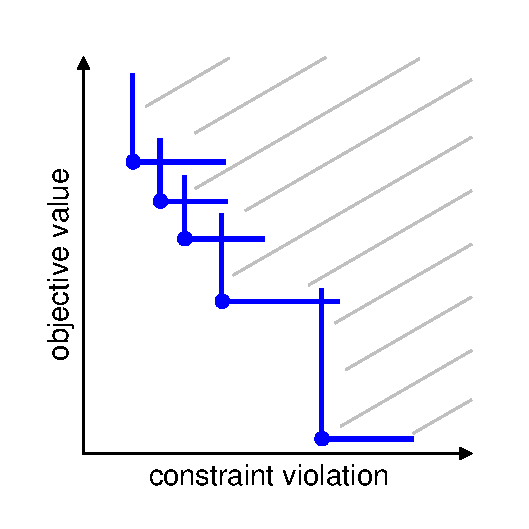
\includegraphics[width=.3\textwidth]{images/filter}
  \caption{Depiction of filter method.}
  \label{fig:filter}
\end{wrapfigure}
When a surrogate optimization is completed and the approximate
solution has been validated, then the decision must be made to either
accept or reject the step.  The traditional approach is to base this
decision on the value of the trust region ratio, as outlined
previously in Table~\ref{tab:rho_k}.  An alternate approach is to
utilize a filter method~\cite{Fle02}, which does not require
penalty parameters or Lagrange multiplier estimates.  The basic idea
in a filter method is to apply the concept of Pareto optimality to the
objective function and constraint violations and only accept an
iterate if it is not dominated by any previous
iterate. Mathematically, a new iterate is not dominated if at least
one of the following:
\begin{equation}
{\rm either~~~} f < f^{(i)} {\rm ~~~or~~~} c < c^{(i)}
%  if (new_f >= filt_f && new_g >= filt_g)
%    return false;            // new point is dominated: reject iterate
%  else if (new_f < filt_f && new_g < filt_g)
%    rm_list.insert(filt_it); // old pt dominated by new: queue for removal
\end{equation}
is true for all $i$ in the filter, where $c$ is a selected norm of the
constraint violation.  This basic description can be augmented with
mild requirements to prevent point accumulation and assure
convergence, known as a slanting filter~\cite{Fle02}.
Figure~\ref{fig:filter} illustrates the filter concept, where
objective values are plotted against constraint violation for accepted
iterates (blue circles) to define the dominated region (denoted by the
gray lines). A filter method relaxes the common enforcement of
monotonicity in constraint violation reduction and, by allowing more
flexibility in acceptable step generation, often allows the algorithm
to be more efficient.
% Note: filter method idea could allow even more flexibility with
% elimination of the reduction of individual constraint violations
% into a single norm.  That is, the Pareto concept could be
% extended to N_con + 1 dimensions.  However, without another
% mechanism to enforce violation reduction, the algorithm could
% easily generate steps that are acceptable to the filter but which
% diverge in constraint violation.

The use of a filter method is compatible with any of the SBO
formulations in Eqs.~\ref{eq:NLP_SBO_TRAL}--\ref{eq:NLP_SBO_direct}.
%; however, it is particularly attractive for the latter since the only
%remaining purpose for a merit function is for managing trust region
%expansion/retention/contraction when the filter accepts a step.
%If alternate logic can be developed
%for that portion, then the entire SBO algorithm can become penalty and
%multiplier free.  In~\cite{Fle02}, for example, trust
%region updates are less structured than in Table~\ref{tab:rho_k} and
%only basic logic is provided (no $\rho^k$ is used).

\section{Merit functions} \label{sbm:sblm_con_merit}

%Merit functions are used in the trust region ratio calculations 
%for sizing subsequent trust regions.  They may also be used for the
%surrogate objective function as described in~\cite{Rod98,Ale00,Per04b},
%which has the advantage of better synchronizing the trust region ratios
%with the approximate optimization steps, but which has the disadvantage
%that it can slow convergence.

The merit function $\Phi({\bf x})$ used in
Eqs.~\ref{eq:NLP_SBO_TRAL}-\ref{eq:NLP_SBO_SQP},\ref{eq:rho_phi_k} may be
selected to be a penalty function, an adaptive penalty function, a
Lagrangian function, or an augmented Lagrangian function.  In each of
these cases, the more flexible inequality and equality constraint
formulations with two-sided bounds and targets
(Eqs.~\ref{eq:NLP_standard},\ref{eq:NLP_SBO_TRAL2}-\ref{eq:NLP_SBO_direct}), 
have been converted to a standard form of ${\bf g}({\bf x}) \le 0$ and
${\bf h}({\bf x}) = 0$ (in
Eqs.~\ref{eq:penalty_merit},\ref{eq:lag_merit}-\ref{eq:lls_lambda}).
The active set of inequality constraints is denoted as ${\bf g}^+$.

The penalty function employed in this paper uses a quadratic penalty
with the penalty schedule linked to SBO iteration number
\begin{eqnarray}
\Phi({\bf x}, r_p) & = & f({\bf x})
%+ \sum_{i=1}^{n_g} r_p (g_i^+({\bf x}))^2
%+ \sum_{i=1}^{n_h} r_p (h_i^+({\bf x}))^2
+ r_p {\bf g}^+({\bf x})^T {\bf g}^+({\bf x})
+ r_p {\bf h}({\bf x})^T {\bf h}({\bf x}) \label{eq:penalty_merit} \\
r_p & = & e^{(k + {\rm offset})/10} % static offset = 21 gives r_p ~ 8 for k = 0
\label{eq:exp_rp}
\end{eqnarray}
The adaptive penalty function is identical in form to
Eq.~\ref{eq:penalty_merit}, but adapts $r_p$ using monotonic increases
in the iteration offset value in order to accept any iterate that
reduces the constraint violation.

The Lagrangian merit function is
\begin{equation}
\Phi({\bf x}, \mbox{\boldmath $\lambda$}_g, \mbox{\boldmath
$\lambda$}_h) = f({\bf x})
%+ \sum_{i=1}^{n_g} (\lambda_i g_i({\bf x})
%+ \sum_{i=1}^{n_h} (\lambda_i h_i({\bf x})
+ \mbox{\boldmath $\lambda$}_g^T {\bf g}^+({\bf x})
+ \mbox{\boldmath $\lambda$}_h^T {\bf h}({\bf x}) \label{eq:lag_merit}
\end{equation}
for which the Lagrange multiplier estimation is discussed in
Section~\ref{sbm:sblm_con_hard}.
% Defer this?:
Away from the optimum, it is possible for the least squares estimates
of the Lagrange multipliers for active constraints to be zero, which
equates to omitting the contribution of an active constraint from the
merit function.  This is undesirable for tracking SBO progress, so
usage of the Lagrangian merit function is normally restricted to
approximate subproblems and hard convergence assessments.

The augmented Lagrangian employed in this paper follows the sign
conventions described in~\cite{Van84}
\begin{eqnarray}
\Phi({\bf x}, \mbox{\boldmath $\lambda$}_{\psi}, \mbox{\boldmath
$\lambda$}_h, r_p) & = & f({\bf x})
%+ \sum_{i=1}^{n_g} (\lambda_i g_i({\bf x}) + r_p (g_i^+({\bf x}))^2)
%+ \sum_{i=1}^{n_h} (\lambda_i h_i({\bf x}) + r_p (h_i^+({\bf x}))^2)
+ \mbox{\boldmath $\lambda$}_{\psi}^T \mbox{\boldmath $\psi$}({\bf x})
+ r_p \mbox{\boldmath $\psi$}({\bf x})^T \mbox{\boldmath $\psi$}({\bf x})
+ \mbox{\boldmath $\lambda$}_h^T {\bf h}({\bf x})
+ r_p {\bf h}({\bf x})^T {\bf h}({\bf x}) \label{eq:aug_lag_merit} \\
\psi_i & = & \max\left\{g_i, -\frac{\lambda_{\psi_i}}{2r_p}\right\}
\label{eq:aug_lag_psi}
\end{eqnarray}
where {\boldmath $\psi$}({\bf x}) is derived from the elimination of
slack variables for the inequality constraints.  In this case, simple
zeroth-order Lagrange multiplier updates may be used:
\begin{eqnarray}
\mbox{\boldmath $\lambda$}_{\psi}^{k+1} & = & \mbox{\boldmath
$\lambda$}_{\psi}^k + 2r_p\mbox{\boldmath $\psi$}({\bf x})
\label{eq:lambda_psi} \\ 
\mbox{\boldmath $\lambda$}_h^{k+1} & = & \mbox{\boldmath $\lambda$}_h^k 
+ 2 r_p {\bf h}({\bf x})
\label{eq:lambda_h}
\end{eqnarray}
The updating of multipliers and penalties is carefully
orchestrated~\cite{Con00} to drive reduction in constraint
violation of the iterates.  The penalty updates can be more
conservative than in Eq.~\ref{eq:exp_rp}, often using an infrequent
application of a constant multiplier rather than a fixed exponential
progression.

%As mentioned previously, a goal for the formulation in
%Eq.~\ref{eq:NLP_SBO_direct} is to employ a penalty and multiplier free
%approach for the merit function and/or trust region logic.  A
%Lagrangian merit function is penalty free and a penalty merit function
%is multiplier free, but no merit functions to this point are both.
%One concept~\cite{Giu00} is to bypass the need for a merit function by
%forming a set of trust region ratios, one for each surrogate function
%(${\hat f}$, ${\hat g}_i$, and ${\hat h}_j$).  In this case, a single
%ratio could be determined from the minimum (or average, norm, etc.) of
%the set,
% -----
%The weakness of this approach is one of scaling near optimality/balancing 
%optimality and feasibility: when constraint values are near zero, the 
%feasibility trust region ratios are less important than the optimality 
%trust region ratios.  This is naturally captured in merit function approaches.
% -----
%or a composite step approach could be used with different trust region
%sizes for the constraint reduction and objective reduction
%subproblems~\cite{Ale00}.  Another concept is to utilize a
%merit function derived from the filter concept using, for example, metrics
%of filter area swept out by accepted iterates.  This concept will be 
%investigated further in future work.
%Initial concepts for swept filter area have issues with potential 
%unboundedness, but will be investigated further in future work.

\section{Convergence assessment} \label{sbm:sblm_con_hard}

To terminate the SBO process, hard and soft convergence metrics are
monitored.  It is preferable for SBO studies to satisfy hard
convergence metrics, but this is not always practical (e.g., when
gradients are unavailable or unreliable).  Therefore, simple soft
convergence criteria are also employed which monitor for diminishing
returns (relative improvement in the merit function less than a
tolerance for some number of consecutive iterations).
% Note: soft convergence is not discussed in \cite{Giu00} (and can't be cited)

To assess hard convergence, one calculates the norm of the projected
gradient of a merit function whenever the feasibility tolerance is
satisfied.  The best merit function for this purpose is the Lagrangian
merit function from Eq.~\ref{eq:lag_merit}.  This requires a least
squares estimation for the Lagrange multipliers that best minimize the
projected gradient:
\begin{equation}
\nabla_x \Phi({\bf x}, \mbox{\boldmath $\lambda$}_g, \mbox{\boldmath
$\lambda$}_h) = \nabla_x f({\bf x})
%+ \sum_{i=1}^{n_g} (\lambda_i g_i({\bf x})
%+ \sum_{i=1}^{n_h} (\lambda_i h_i({\bf x})
+ \mbox{\boldmath $\lambda$}_g^T \nabla_x {\bf g}^+({\bf x}) +
\mbox{\boldmath $\lambda$}_h^T \nabla_x {\bf h}({\bf x})
\label{eq:lag_merit_grad}
\end{equation}
where gradient portions directed into active global variable bounds
have been removed.  This can be posed as a linear least squares
problem for the multipliers:
\begin{equation}
{\bf A} \mbox{\boldmath $\lambda$} = -\nabla_x f \label{eq:lls_lambda}
\end{equation}
where ${\bf A}$ is the matrix of active constraint gradients,
$\mbox{\boldmath $\lambda$}_g$ is constrained to be non-negative, and
$\mbox{\boldmath $\lambda$}_h$ is unrestricted in sign.  To estimate
the multipliers using non-negative and bound-constrained linear least
squares, the NNLS and BVLS routines~\cite{Law74} from NETLIB are used,
respectively.

\section{Constraint relaxation} \label{sbm:sblm_con_relax}

% trConstraintRelax may be COMPOSITE\_STEP or HOMOTOPY.  

The goal of constraint relaxation is to achieve efficiency through the
balance of feasibility and optimality when the trust region
restrictions prevent the location of feasible solutions to constrained
approximate subproblems
(Eqs.~\ref{eq:NLP_SBO_TRAL2}-\ref{eq:NLP_SBO_direct}, and other
formulations from rows 2-3 in Table~\ref{tab:sbo_subprob}).  The SBO
algorithm starting from infeasible points will commonly generate
iterates which seek to satisfy feasibility conditions without regard
to objective reduction~\cite{Per04b}.

One approach for achieving this balance is to use {\em relaxed
constraints} when iterates are infeasible with respect to the
surrogate constraints.  We follow Perez, Renaud, and
Watson~\cite{Per04a}, and use a {\em global homotopy} mapping the
relaxed constraints and the surrogate constraints.  For formulations
in Eqs.~\ref{eq:NLP_SBO_TRAL2} and~\ref{eq:NLP_SBO_direct} (and others
from row 3 in Table~\ref{tab:sbo_subprob}), the relaxed constraints
are defined from
\begin{eqnarray}
{\bf {\tilde g}}^k({\bf x}, \tau) &=& {\bf {\hat g}}^k({\bf x}) + 
(1-\tau){\bf b}_{g} \label{eq:relaxed_ineq}\\
{\bf {\tilde h}}^k({\bf x}, \tau) &=& {\bf {\hat h}}^k({\bf x}) + 
(1-\tau){\bf b}_{h} \label{eq:relaxed_eq}
\end{eqnarray}
For Eq.~\ref{eq:NLP_SBO_SQP} (and others from row 2 in
Table~\ref{tab:sbo_subprob}), the original surrogate constraints 
${\bf {\hat g}}^k({\bf x})$ and ${\bf {\hat h}}^k({\bf x})$ in
Eqs.~\ref{eq:relaxed_ineq}-\ref{eq:relaxed_eq} are replaced with 
their linearized forms (${\bf {\hat g}}^k({\bf x}^k_c) + 
\nabla {\bf {\hat g}}^k({\bf x}^k_c)^T ({\bf x} - {\bf x}^k_c)$ 
and ${\bf {\hat h}}^k({\bf x}^k_c) + \nabla {\bf {\hat h}}^k({\bf x}^k_c)^T 
({\bf x} - {\bf x}^k_c)$, respectively).  The approximate subproblem
is then reposed using the relaxed constraints as
\begin{eqnarray}
{\rm minimize } & {\hat f^k}({\bf x})~~{\rm or}~~{\hat \Phi}^k({\bf x})
\nonumber \\
{\rm subject\  to } 
  & {\bf g}_l \le {\bf {\tilde g}}^k({\bf x},\tau^k) \le {\bf g}_u \nonumber \\
  &               {\bf {\tilde h}}^k({\bf x},\tau^k) = {\bf h}_t \nonumber \\
  & {\parallel {\bf x} - {\bf x}^k_c \parallel}_\infty \le \Delta^k
% & {\bf x}_l \le {\bf x} \le {\bf x}_u \nonumber\\
%  & 0 \le \tau \le 1 
\label{eq:NLP_relaxed}
\end{eqnarray}
in place of the corresponding subproblems in 
Eqs.~\ref{eq:NLP_SBO_TRAL2}-\ref{eq:NLP_SBO_direct}. Alternatively, 
since the relaxation terms are constants for the $k^{th}$ iteration, 
it may be more convenient for the implementation to constrain 
${\bf {\hat g}}^k({\bf x})$ and ${\bf {\hat h}}^k({\bf x})$ (or their
linearized forms) subject to relaxed bounds and targets 
(${\bf {\tilde g}}_l^k$, ${\bf {\tilde g}}_u^k$, ${\bf {\tilde h}}_t^k$).  
The parameter $\tau$ is the homotopy parameter controlling the extent of 
the relaxation: when $\tau=0$, the constraints are fully relaxed, and 
when $\tau=1$, the surrogate constraints are recovered.  The vectors 
${\bf b}_{g}, {\bf b}_{h}$ are chosen so that the starting point, 
${\bf x}^0$, is feasible with respect to the fully relaxed constraints:
% NOTE: these _could_ need updating in the case of global data fits
\begin{eqnarray}
&{\bf g}_l \le {\bf {\tilde g}}^0({\bf x}^0, 0) \le {\bf g}_u \\
&{\bf {\tilde h}}^0({\bf x}^0, 0) =  {\bf h}_t
\end{eqnarray}

At the start of the SBO algorithm, $\tau^0=0$ if ${\bf x}^0$ is
infeasible with respect to the unrelaxed surrogate constraints;
otherwise $\tau^0=1$ (i.e., no constraint relaxation is used).  At the
start of the $k^{th}$ SBO iteration where $\tau^{k-1} < 1$, $\tau^k$
is determined by solving the subproblem
\begin{eqnarray}
{\rm maximize } & \tau^k \nonumber \\
{\rm subject\  to } 
  & {\bf g}_l \le {\bf {\tilde g}}^k({\bf x},\tau^k) \le {\bf g}_u \nonumber \\
  &               {\bf {\tilde h}}^k({\bf x},\tau^k) = {\bf h}_t \nonumber \\
  & {\parallel {\bf x} - {\bf x}^k_c \parallel}_\infty \le \Delta^k \nonumber\\
% & {\bf x}_l \le {\bf x} \le {\bf x}_u \nonumber\\
  & \tau^k \ge 0 \label{eq:tau_max}
\end{eqnarray}
% NOTE 2: 
starting at $({\bf x}^{k-1}_*, \tau^{k-1})$, and then adjusted as follows:
\begin{equation}
\tau^k = \min\left\{1,\tau^{k-1} + \alpha
\left(\tau^{k}_{\max}-\tau^{k-1}\right)\right\}
\end{equation}
The adjustment parameter $0 < \alpha < 1$ is chosen so that that the
feasible region with respect to the relaxed constraints has positive
volume within the trust region.  Determining the optimal value for
$\alpha$ remains an open question and will be explored in future work.

After $\tau^k$ is determined using this procedure, the problem in
Eq.~\ref{eq:NLP_relaxed} is solved for ${\bf x}^k_\ast$.
% Note: could just use $\tau^k$ in previous equations above
If the step is accepted, then the value of $\tau^k$ is 
updated using the current iterate ${\bf x}^k_\ast$ and the validated
constraints ${\bf g}({\bf x}^k_\ast)$ and ${\bf h}({\bf x}^k_\ast)$:
\begin{eqnarray}
\tau^{k} & = \min\left\{1,\min_i \tau_i , \min_j \tau_j \right\} \\
\rm{where}~~
\tau_i & = 1 + \frac{\min \left\{g_i({\bf x}^k_\ast) - g_{l_{i}}, 
g_{u_{i}} - g_i({\bf x}^k_\ast)\right\}}{b_{g_{i}}} \\ 
\tau_j & = 1 - \frac{| h_j({\bf x}^k_\ast) - h_{t_{j}} |}{b_{h_{j}}}
\end{eqnarray}
%\begin{align}
%\tau^{k} & = \min\left\{1,\min_i \tau_i , \min_j \tau_j \right\} \; ,\\
%\intertext{where}
%\tau_i & = \frac{\min \left\{\hat g_i({\bf x}^k) - ({\bf g}_l)_i, 
%({\bf g}_u)_i - \hat g_i({\bf x}^k)\right\}}{b_i^{g}} + 1\\ 
%\tau_j & = \frac{- | \hat h_j({\bf x}^k) - ({\bf h}_t)_j |}{b_j^{h}} + 1 \; .
%\end{align}

\begin{wrapfigure}{r}{.35\textwidth}
  \centering
  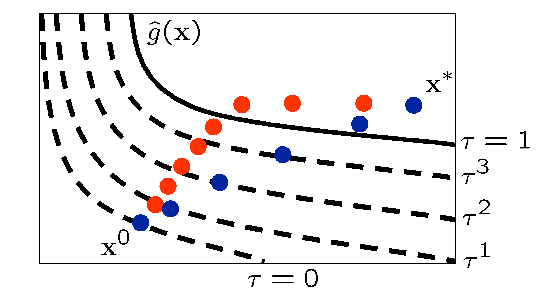
\includegraphics[width=.35\textwidth]{images/tau_updates}
  \caption{Illustration of SBO iterates using surrogate (red) and
  relaxed (blue) constraints.}
  \label{fig:constr_relax}
\end{wrapfigure}
Figure~\ref{fig:constr_relax} illustrates the SBO algorithm on a
two-dimensional problem with one inequality constraint starting from
an infeasible point, ${\bf x}^0$.  The minimizer of the problem is
denoted as ${\bf x}^*$.  Iterates generated using the surrogate
constraints are shown in red, where feasibility is achieved first, and
then progress is made toward the optimal point.  The iterates
generated using the relaxed constraints are shown in blue, where a
balance of satisfying feasibility and optimality has been achieved,
leading to fewer overall SBO iterations.
%\begin{figure}[ht!]
%\epsfxsize 3in \centerline{\epsfbox{tau_updates.eps}}
%\caption{Example SBO iterates using surrogate (red) and relaxed (blue)
%constraints.}
%\label{fig:constr_relax}
%\end{figure}

The behavior illustrated in Fig.~\ref{fig:constr_relax} is an example
where using the relaxed constraints over the surrogate constraints may
improve the overall performance of the SBO algorithm by reducing the
number of iterations performed.  This improvement comes at the cost of
solving the minimization subproblem in Eq.~\ref{eq:tau_max}, which can
be significant in some cases (i.e., when the cost of evaluating 
${\bf {\hat g}}^k({\bf x})$ and ${\bf {\hat h}}^k({\bf x})$ is not
negligible, such as with multifidelity or ROM surrogates).  As shown
in the numerical experiments involving the Barnes problem presented 
in ~\cite{Per04a}, 
the directions toward constraint violation
reduction and objective function reduction may be in opposing
directions.  In such cases, the use of the relaxed constraints may
result in an {\em increase} in the overall number of SBO iterations
since feasibility must ultimately take precedence.
